\chapter{La ricorsività}
{ }\hfill\textbf{Livello:} Medio\\ \\

La programmazione in \logo\ spesso usa una tecnica chiamata ricorsività. In questo capitolo esploreremo la ricorsività con semplici esempi e disegneremo alla fine una curva frattale chiamata ``fiocco di neve di Van Koch''.\\
Prima di tutto:
\begin{center}
	\textbf{Una procedura è ricorsiva se invoca se stessa}
\end{center}


\section{Nell'area di disegno}
\subsection{Un primo semplice esempio}
\begin{lstlisting}[caption="Una semplice procedura ricorsiva"]
Per ex1
	DX 1
	ex1
Fine  
\end{lstlisting}
Questa procedura è ricorsiva perché la procedura \texttt{ex1} è invocata nell'ultima riga della medesima procedura. Durante l'esecuzione osserviamo che la tartaruga ruota su stessa verso destra all'infinito. Per interrompere il programma dobbiamo cliccare il bottone di STOP.


\subsection{Un secondo esempio}
Per il secondo esempio impariamo tre nuove primitive:
\begin{itemize}
	\item \texttt{Aspetta numero}\hspace {4cm } \textcolor{red}{ \texttt{Aspetta 60}}\\
	Mette in pausa il programma per $numero / 60$ secondi. \\
	Per esempio \texttt{Aspetta 120} metterà in pausa il programma per 2 secondi.
	\item \texttt{CancellaPenna}\hspace {4cm } \textcolor{red}{{CancellaPenna}}\\
	Quando la tartaruga si sposta, cancella tutto ciò che incontra invece di disegnare.
	\item \texttt{PennaDisegno}\hspace {4cm } \textcolor{red}{PennaDisegno}\\
	Ritorna alla modalità classica di disegno.
\end{itemize}

\begin{lstlisting}[caption="La lancetta dei secondi di un orologio"]
Per ex2
	Av 200 CancellaPenna Aspetta 60
	In 200 PennaDisegno DX 6
	ex2
Fine
\end{lstlisting}
Il programma ripete la stessa procedura ogni secondo ottenendo i secondi di un orologio.




\section{Nell'area dello storico dei comandi}
\subsection{Un primo semplice esempio}

\noindent La primitiva \texttt{Stampa} visualizza del testo nell'area dello storico dei comandi. \texttt{Stampa} si aspetta un argomento, un elenco o una parola.\\
Per esempio: \texttt{Stampa \textquotedbl hello} \texttt{Stampa [Essere o non essere]} (non dimenticare le virgolette \textquotedbl quando vuoi scrivere solo una parola).
\begin{lstlisting}[caption="Stampare un elenco infinito di numeri"]
Per ex3 :n
	Stampa :n
	ex3 :n+1
Fine
\end{lstlisting}
Invoca la procedura \texttt{ex3 0} e ferma il programma con il bottone di STOP.\\
Come esercizio modifica il programma per visualizzare i numeri con un intervallo di 2.\\

Vogliamo ora visualizzare tutti i numeri interi maggiori di 100 che sono divisibili per 5. Dobbiamo solo modificare il programma così:
\begin{lstlisting}[caption="Stampare un elenco di numeri divisibili per 5"]
Per ex3 :n
	Stampa :n
	ex3 :n+5
end
\end{lstlisting}
e quindi invocare: \texttt{ex3 100}


\subsection{Uscita dalla ricorsione}
Tutti gli esempi precedenti vengono eseguiti all'infinito consumando piano piano tutta la memoria disponibile fino a quando \xlogo\ fermerà il programma. Normalmente, però, la ricorsione viene fermata dal programma stesso quando si verifica una determinata condizione. Esempi di condizioni sono i seguenti esempi:\\
\texttt{Se 2+1=3 [Stampa [è vero]]} \\
\texttt{Se 2+1=4 [Stampa [è vero]][print [è falso]]} \\
\texttt{Se 2+5=7 [Stampa \textquotedbl vero][Stampa \textquotedbl falso]}\\
\\
Se non ti è chiara la sintassi delle condizioni vai alla pagina della primitiva \texttt{Se}. Il seguente esempio modifica il terzo esempio per interrompe la ricorsione al 100-esimo numero.
\begin{lstlisting}[caption="Stampare un elenco di numeri inferiori a 0"]
Per ex3 :n
	Se :n=100 [Ferma]
	Stampa :n
	ex3 :n+1
Fine
\end{lstlisting}
Invoca il programma con \texttt{ex3 0}.\\
Come esercizio puoi modificare il programma per visualizzare numeri interi tra 55 e 350 che sono divisibili per 11.\\




\section{L'esempio di un frattale, il fiocco di neve di Van Koch}
\label{vankoch}
Utilizzando la ricorsione è molto semplice generare in \logo\ alcune semplici curve chiamate frattali in matematica.\\
Questi sono i primi passi per creare la linea spezzata di Van Koch:

\begin{center}
	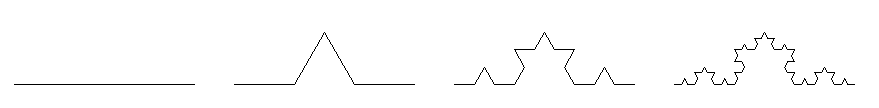
\includegraphics[width=\textwidth]{pics/koch0123.png}
\end{center}

Come primo passo si disegna un segmento di una data lunghezza.\\
Come secondo passo:
\begin{enumerate}
	\item il segmento viene diviso in tre parti uguali.
	\item un triangolo equilatero viene disegnato sul segmento centrale.
	\item infine il segmento centrale viene cancellato.
\end{enumerate}

A questo punto il segmento originario risulterà spezzato in quattro segmenti di lunghezza pari ad $\frac{1}{3}$ di quello originario (terza figura). Il secondo passo viene quindi ripetuto su ciascuno dei quattro segmenti originando 16 segmenti di lunghezza pari ad $\frac{1}{3}$ dei precedenti, ossia $\frac{1}{3} \cdot \frac{1}{3} = \frac{1}{9}$ (quarta figura). Ad ogni  passo la lunghezza dei segmenti si riduce di un fattore 3.\\
\textbf{Importante} Abbiamo scovato la natura ricorsiva dei frattali! \\
Vediamo come impostare concettualmente il programma \logo. Chiamiamo $L_{n,\ell}$ il segmento di lunghezza $\ell$, corrispondente al passo $n$.\\
Per disegnare il segmento:
\begin{enumerate}
	\item Disegniamo $L_{n-1,\ell/3}$
	\item Ruotiamo a sinistra di 60$^{\circ}$
	\item Disegniamo $L_{n-1,\ell/3}$
	\item Ruotiamo a destra di 120$^{\circ}$
	\item Disegniamo $L_{n-1,\ell/3}$
	\item Ruotiamo a sinistra di 60$^{\circ}$
	\item Disegniamo $L_{n-1,\ell/3}$
\end{enumerate}

In \logo, il programma è molto semplice:
\begin{lstlisting}[caption="Procedura ricorsiva per il disegno di un segmento frattale"]
	# :l contiene la lunghezza del segmento
	# :n contiene il numero del passo
to linea :l :n
	Se :n=0 [Av :l] [
	linea :l/3 :n-1 SX 60 linea :l/3 :n-1 DX 120 linea :l/3 :n-1 SX 60 linea :l/3 :n-1
	]
end
\end{lstlisting}
Il programma si invoca come \texttt{linea 50 3}, dove il primo argomento è la lunghezza del segmento originario ed il secondo argomento è il numero di ricorsioni da eseguire. Incredibile il potere della ricorsione!\\
Se disegniamo un triangolo equilatero con tre linee di Van Koch otteniamo uno stupendo fiocco di neve di Van Koch.
\begin{lstlisting}[caption="Fiocco di neve di Van Koch"]
	# :l lunghezza del lato
Per fioccoNeve :l :p
	Ripeti 3[linea :l :p DX 120]
Fine
\end{lstlisting}
Il programma si invoca per esempio con: \texttt{fioccoNeve 200 6}
\begin{center}
	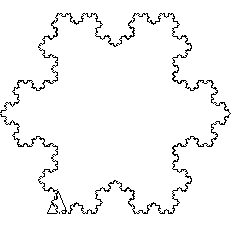
\includegraphics{pics/flocon.png}
\end{center}




\section{Ricorsione con le parole}
Leggi pagina \pageref{liste-prim} per capire come impiegare le primitive \texttt{Parola}, \texttt{Ultimo}, e \texttt{EccettoUltimo, EU}.\\

\subsection{Leggere al contrario le parole}

\begin{lstlisting}[caption="Ricorsione per invertire l'ordine delle lettere in un parola"]
Per invertiParola :m
	Se vuoto? :m [output "]  
	output parola ultimo :m invertiParola eccettoultimo :m
Fine
\end{lstlisting}

Si invoca con \texttt{Stampa invertiParola \textquotedbl Logo}.

\subsection{I palindromi}
Un palindromo è una parola o una frase che si può leggere in entrambi i sensi (esempi: I treni inerti, Etna gigante \textellipsis ). Aggiungiamo una semplice verifica all'esempio precedente per capire se la parola o la frase è palindroma.
\begin{lstlisting}[caption="Verificare se una parola è palindroma"]
# Verifica se la parola :m e' palindroma
Per palindromo :m
	Se :m=invertiParola :m [output vero] [output falso]
Fine
\end{lstlisting}

\subsection{I numeri palindromi}
Anche i numeri possono essere palindromi, per esempio 4884. Infine, un programma per cercare numeri palindromi a partire da un qualsiasi numero (Grazie Olivier SC):
\begin{lstlisting}[caption="Scovare numeri palondromi"]
Per numeroPalindromo :n
	Se palindromo :n [Stampa :n Ferma]
	Stampa (elenco :n "Piu' invertiParola :n "uguale somma :n invertiParola :n)
	numeroPalindromo :n + invertiParola :n 
end
\end{lstlisting} 

Si invoca con \texttt{numeroPalindromo 78}:
\begin{verbatim}
	78 Più 87 uguale 165 
	165 Più 561 uguale 726 
	726 Più 627 uguale 1353 
	1353 Più 3531 uguale 4884 
	4884 
\end{verbatim} 



\section{Calcolo di un numero fattoriale}
\label{factorielle}
Il fattoriale di un numero $n$ è il prodotto dei primi $n$ numeri interi positivi. Per esempio il fattoriale di 5 è definito come: $$5!=5\times4\times3\times2\times1=120$$
In termini matematici se $n$ è un intero positivo: $n!=n\times(n-1)!$. Questa relazione spiega la natura ricorsiva del programma fattoriale:
\begin{lstlisting}[caption="La ricorsività nel calcolo del fattoriale"]
Per fattoriale :n
	Se :n=0[output 1][output :n*fattoriale :n-1]
Fine
\end{lstlisting}

Si invoca con \texttt{Stampa fattoriale 5}.


\section{Calcolo del pi greco per approssimazione}
\label{approx-pi}

Possiamo approssimare il numero pi greco utilizzando la formula:
$$\pi\approx2^k\sqrt{2-\sqrt{2+\sqrt{2+\ldots\sqrt{2+\sqrt2}}}}$$ dove $k$ è il numero di radici quadrate. Maggiore è $k$, migliore risulterà l'approssimazione di pi greco.\\

La formula contiene l'espressione ricorsiva $2+\sqrt{2+\ldots\sqrt{2+\sqrt2}}$, quindi ecco il programma:
\begin{lstlisting}[caption="Approssimazione del valore del pi greco"]
# k e' il numero di radici quadrate
Per approxpi :k
	Stampa [Approssimazione di pi greco:]  
	Stampa (potenza 2 :k) * RadQ (2- RadQ (calc :k-2))
	Stampa "-------------------------
	Stampa [Esatto pi greco:]  Stampa pi
Fine

Per calc :p
	Se :p=0 [output 2][output 2+RadQ calc :p-1]
Fine
\end{lstlisting}

Si invoca con \texttt{approxpi 10}.


Con 10 approssimazioni troviamo i primi 5 decimali! Se vuoi trovare più decimali devi aumentare la precisione aumentando il numero di decimali con la primitiva \texttt{ImpostaDecimali}.
\begin{lstlisting}[caption="Il pi greco con 100 decimali"]
ImpostaDecimali 100
approxpi 100
\end{lstlisting}

E ora abbiamo 39 decimali esatti\textellipsis